\documentclass[../../main.tex]{subfiles}

\begin{document}

    Aufgrund der erhöhten technischen Umsetzungsgeschwindigkeit einer Eingabeleistungsänderung am Diodenlaser versuchen wir zunächst mittels Rasterung über eine konstante Temperatur $T$ Minima in der Funktion $P_{\textit{an}}\mapsto \textit{Tr}(P_{\textit{an}})(T)$ zu finden. Unsere Messergebnisse für $T\in\{22\si{\celsius}, 24\si{\celsius}, 26\si{\celsius}, 28\si{\celsius}, 30\si{\celsius}\}=:\mcT$ sind in Abbildung \ref{fig:1-2:Rasterung22deg} bis \ref{fig:1-2:Rasterung30deg} zu sehen. 
    \begin{figure}
        \centering
        \begin{subfigure}[t]{0.45\textwidth}
            \centering
            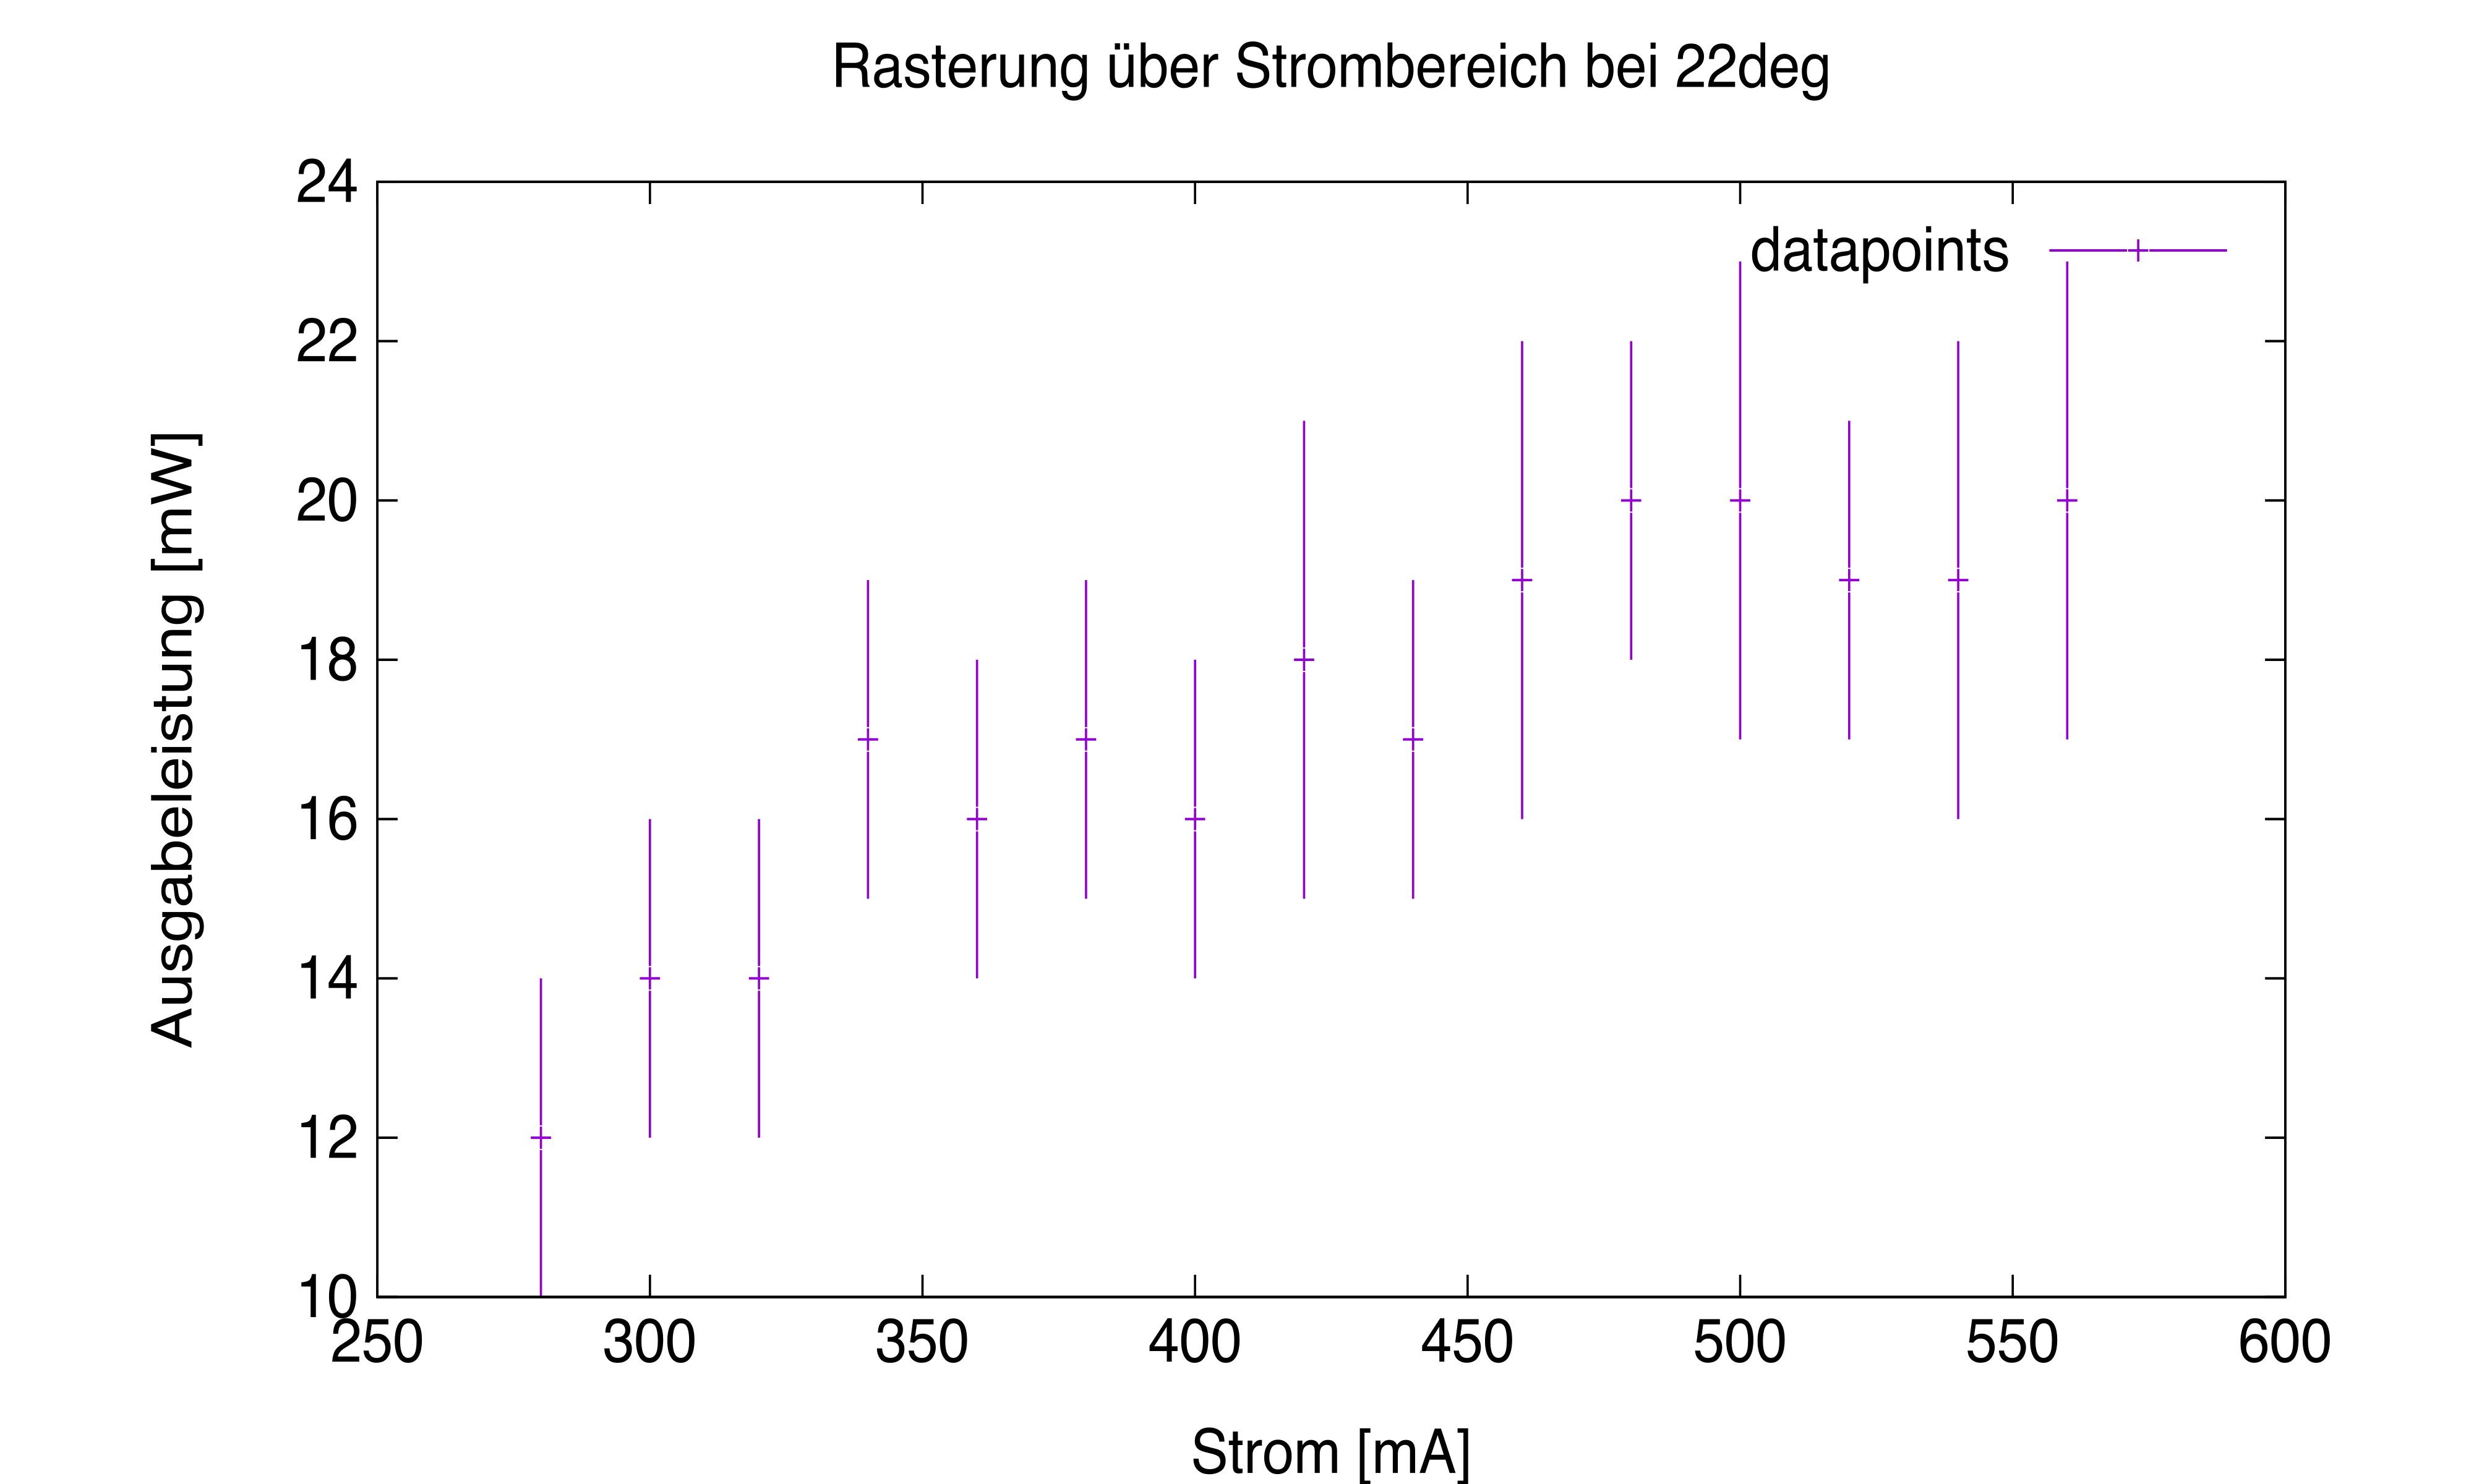
\includegraphics[width=\textwidth]{../../Bilddateien/1-2/Rasterung_22deg.png}
            \caption{Rasterung um $22\si{\celsius}$.}
            \label{fig:1-2:Rasterung22deg}
        \end{subfigure}
        \
        \begin{subfigure}[t]{0.45\textwidth}
            \centering
            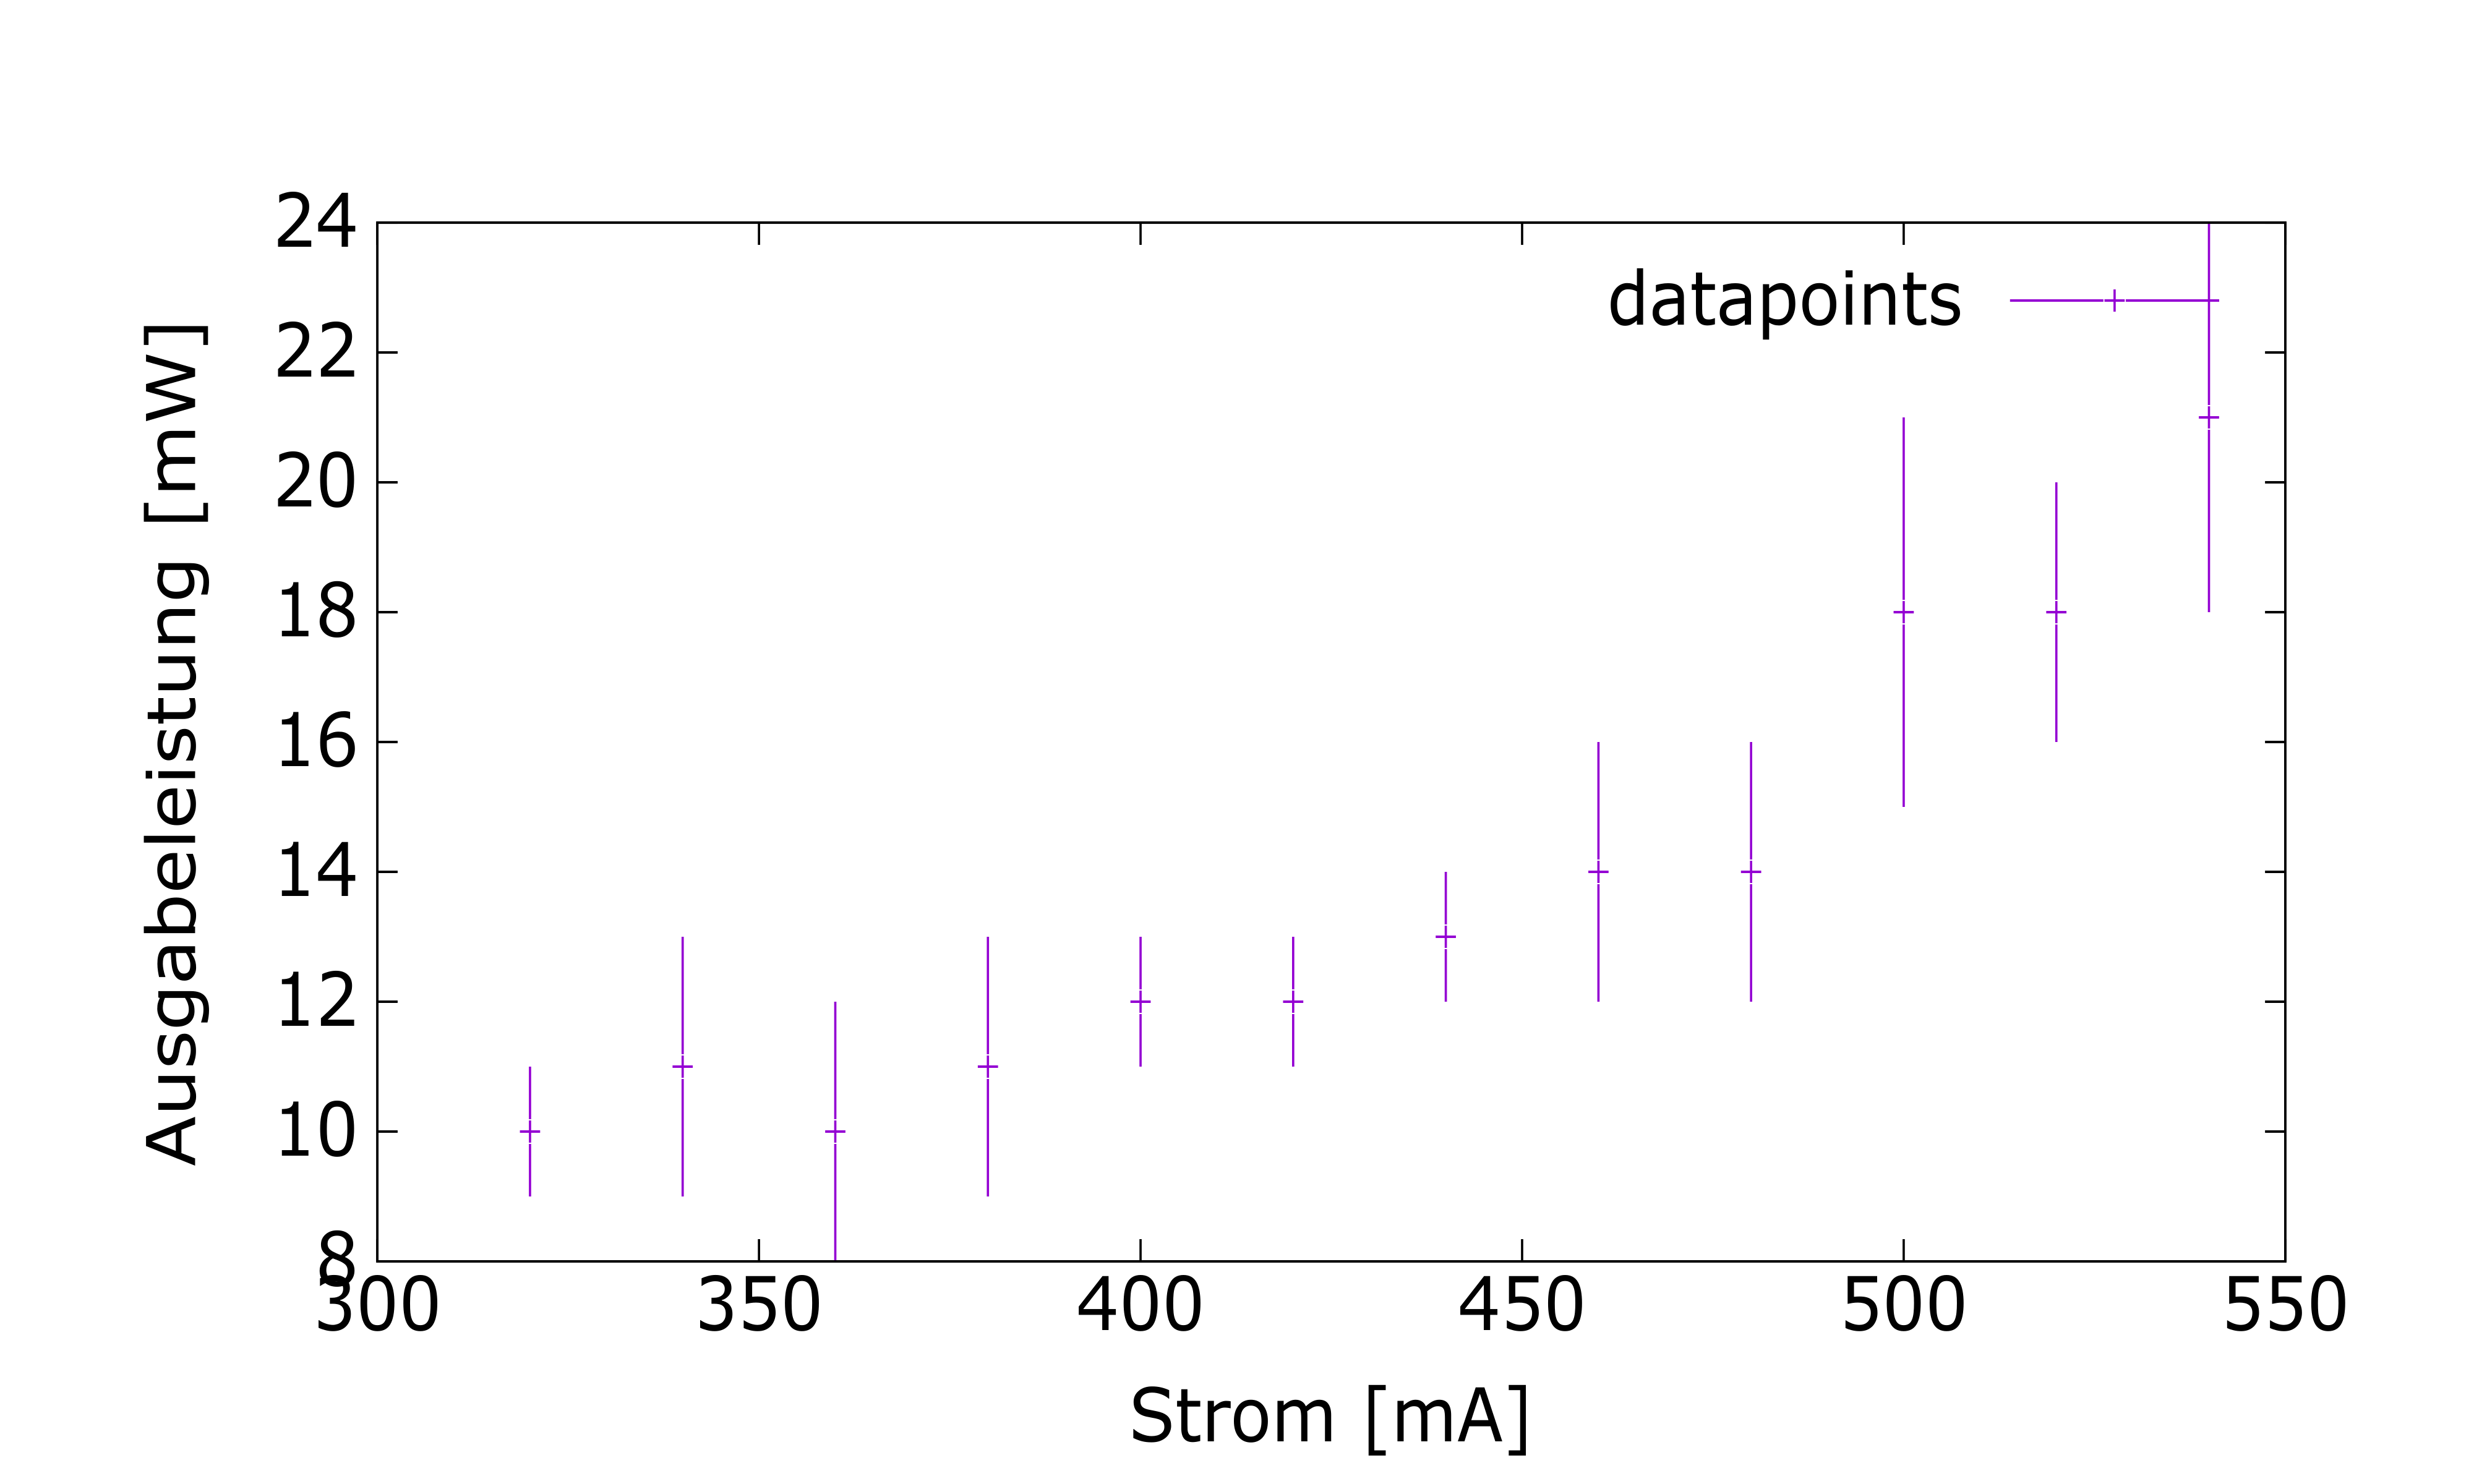
\includegraphics[width=\textwidth]{../../Bilddateien/1-2/Rasterung_24deg.png}
            \caption{Rasterung um $24\si{\celsius}$.}
            \label{fig:1-2:Rasterung24deg}
        \end{subfigure}
        \
        \begin{subfigure}[t]{0.45\textwidth}
            \centering
            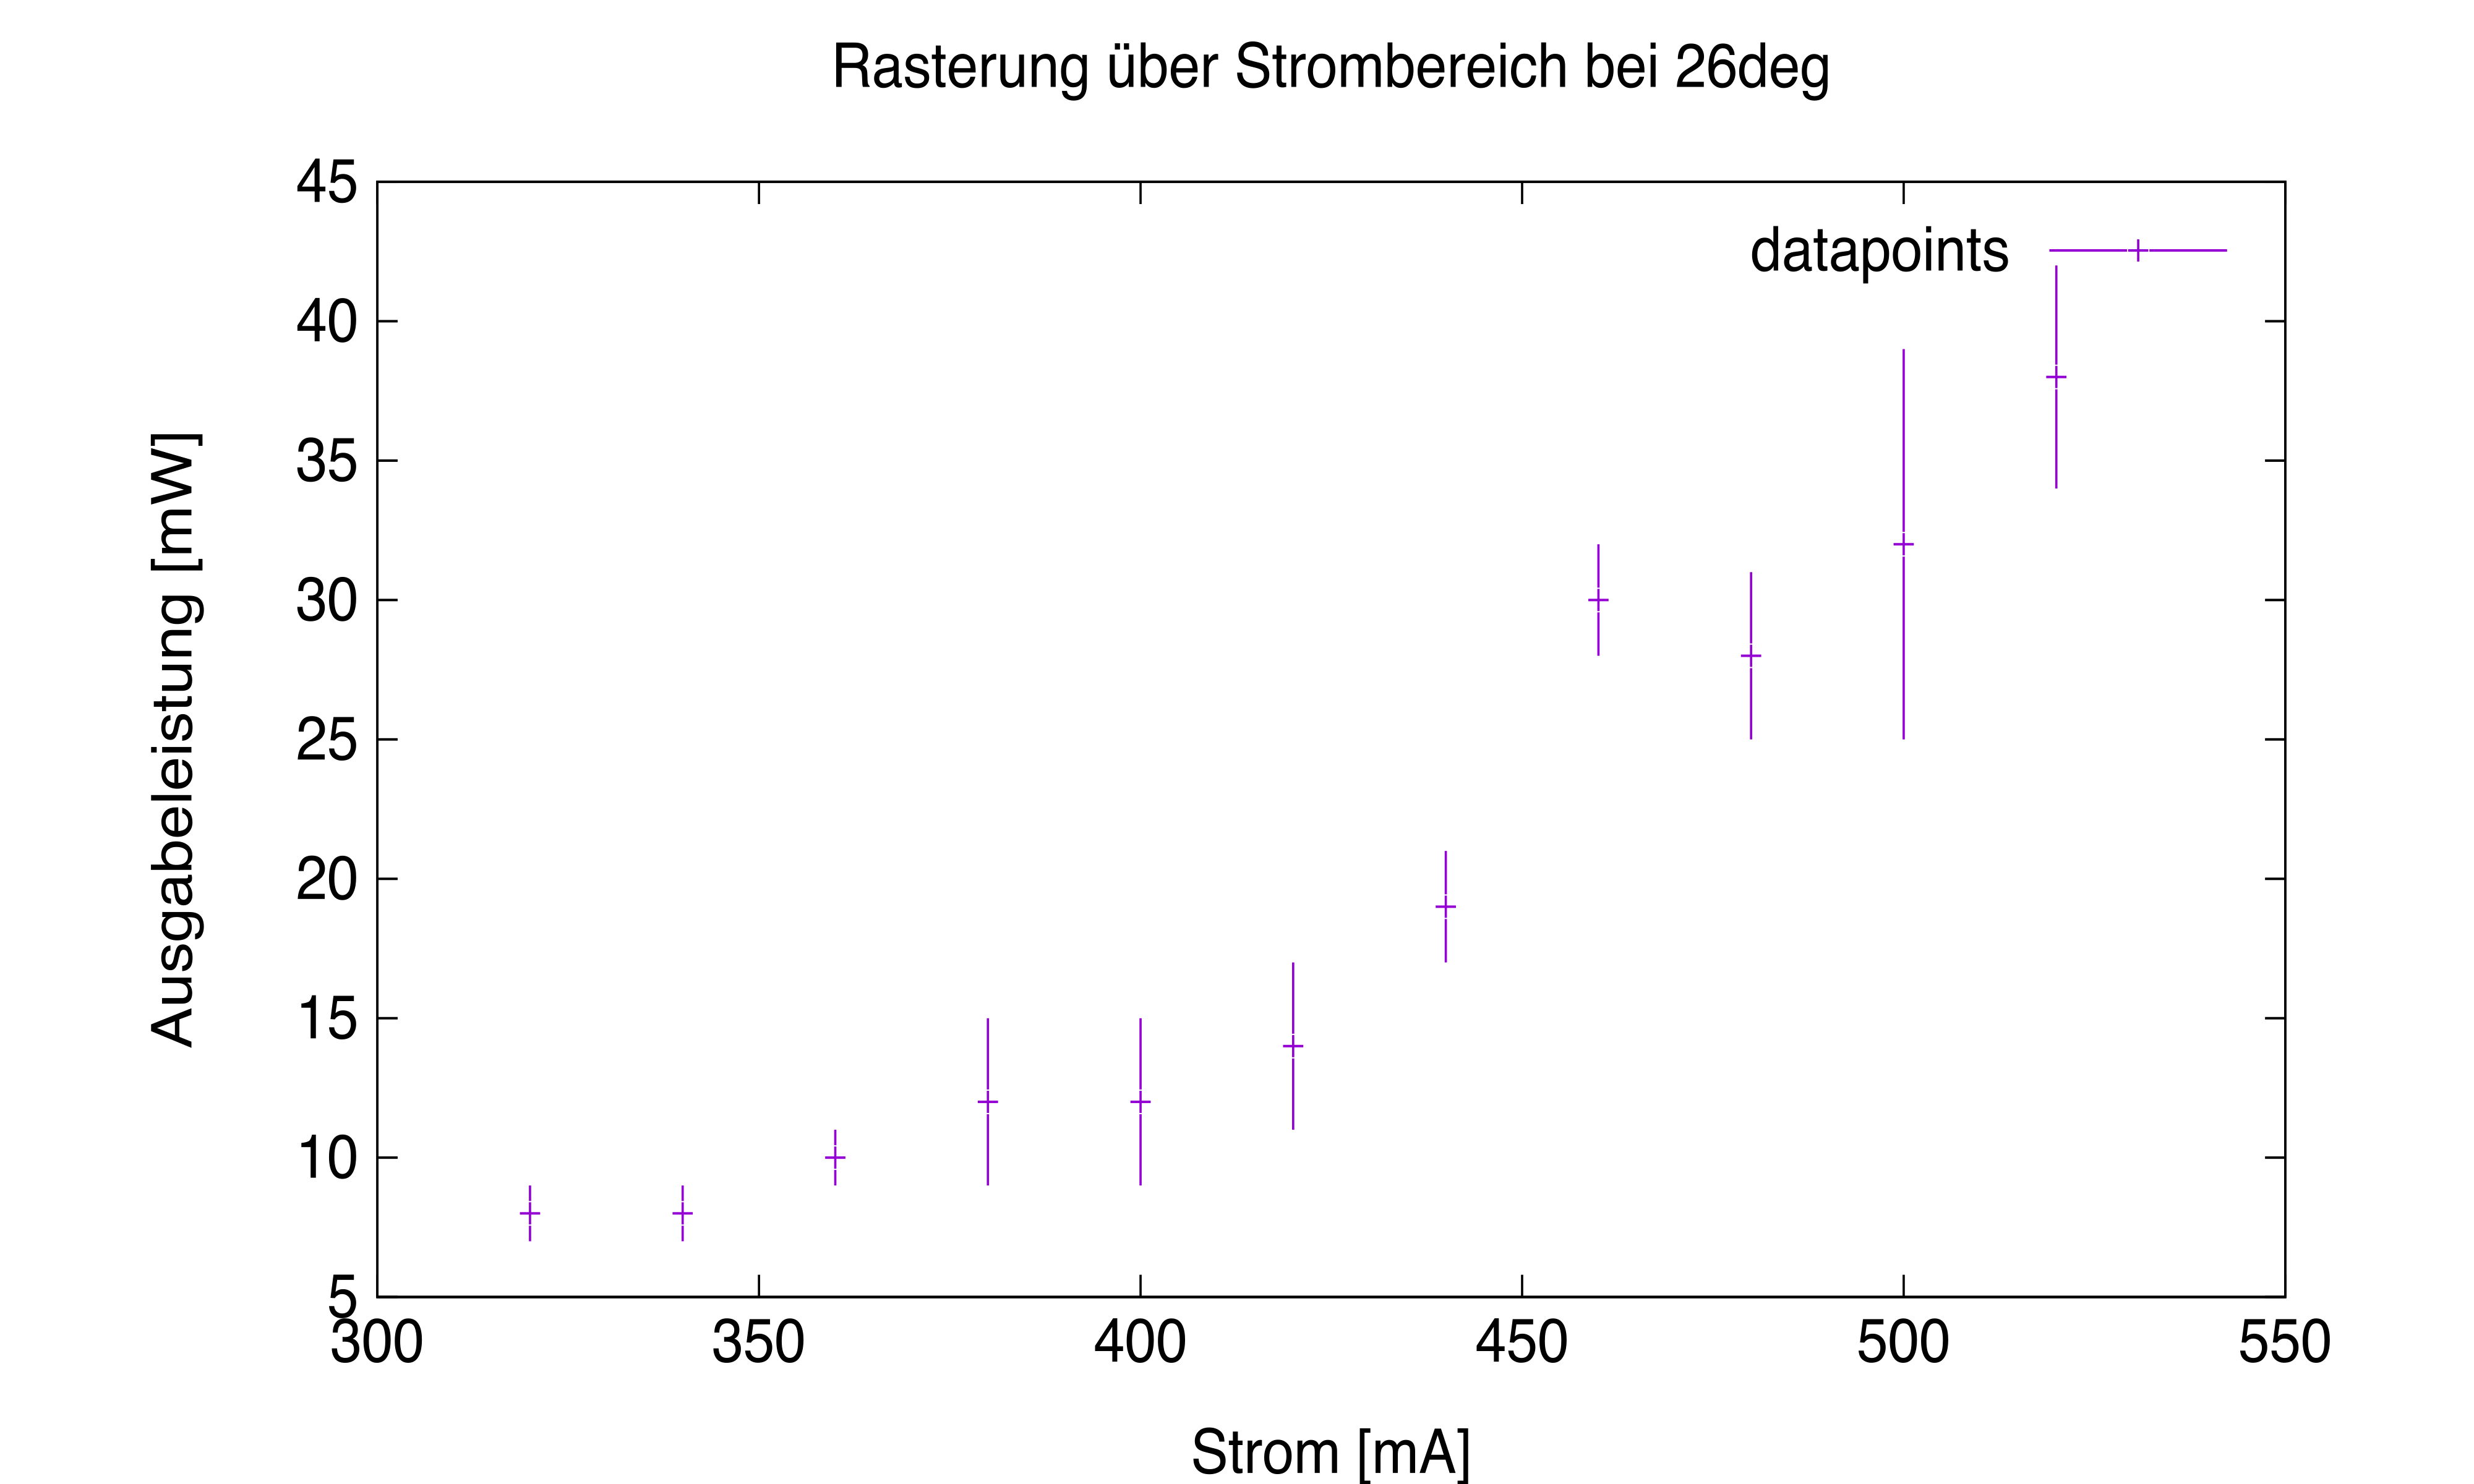
\includegraphics[width=\textwidth]{../../Bilddateien/1-2/Rasterung_26deg.png}
            \caption{Rasterung um $26\si{\celsius}$.}
            \label{fig:1-2:Rasterung26deg}
        \end{subfigure}
        \
        \begin{subfigure}[t]{0.45\textwidth}
            \centering
            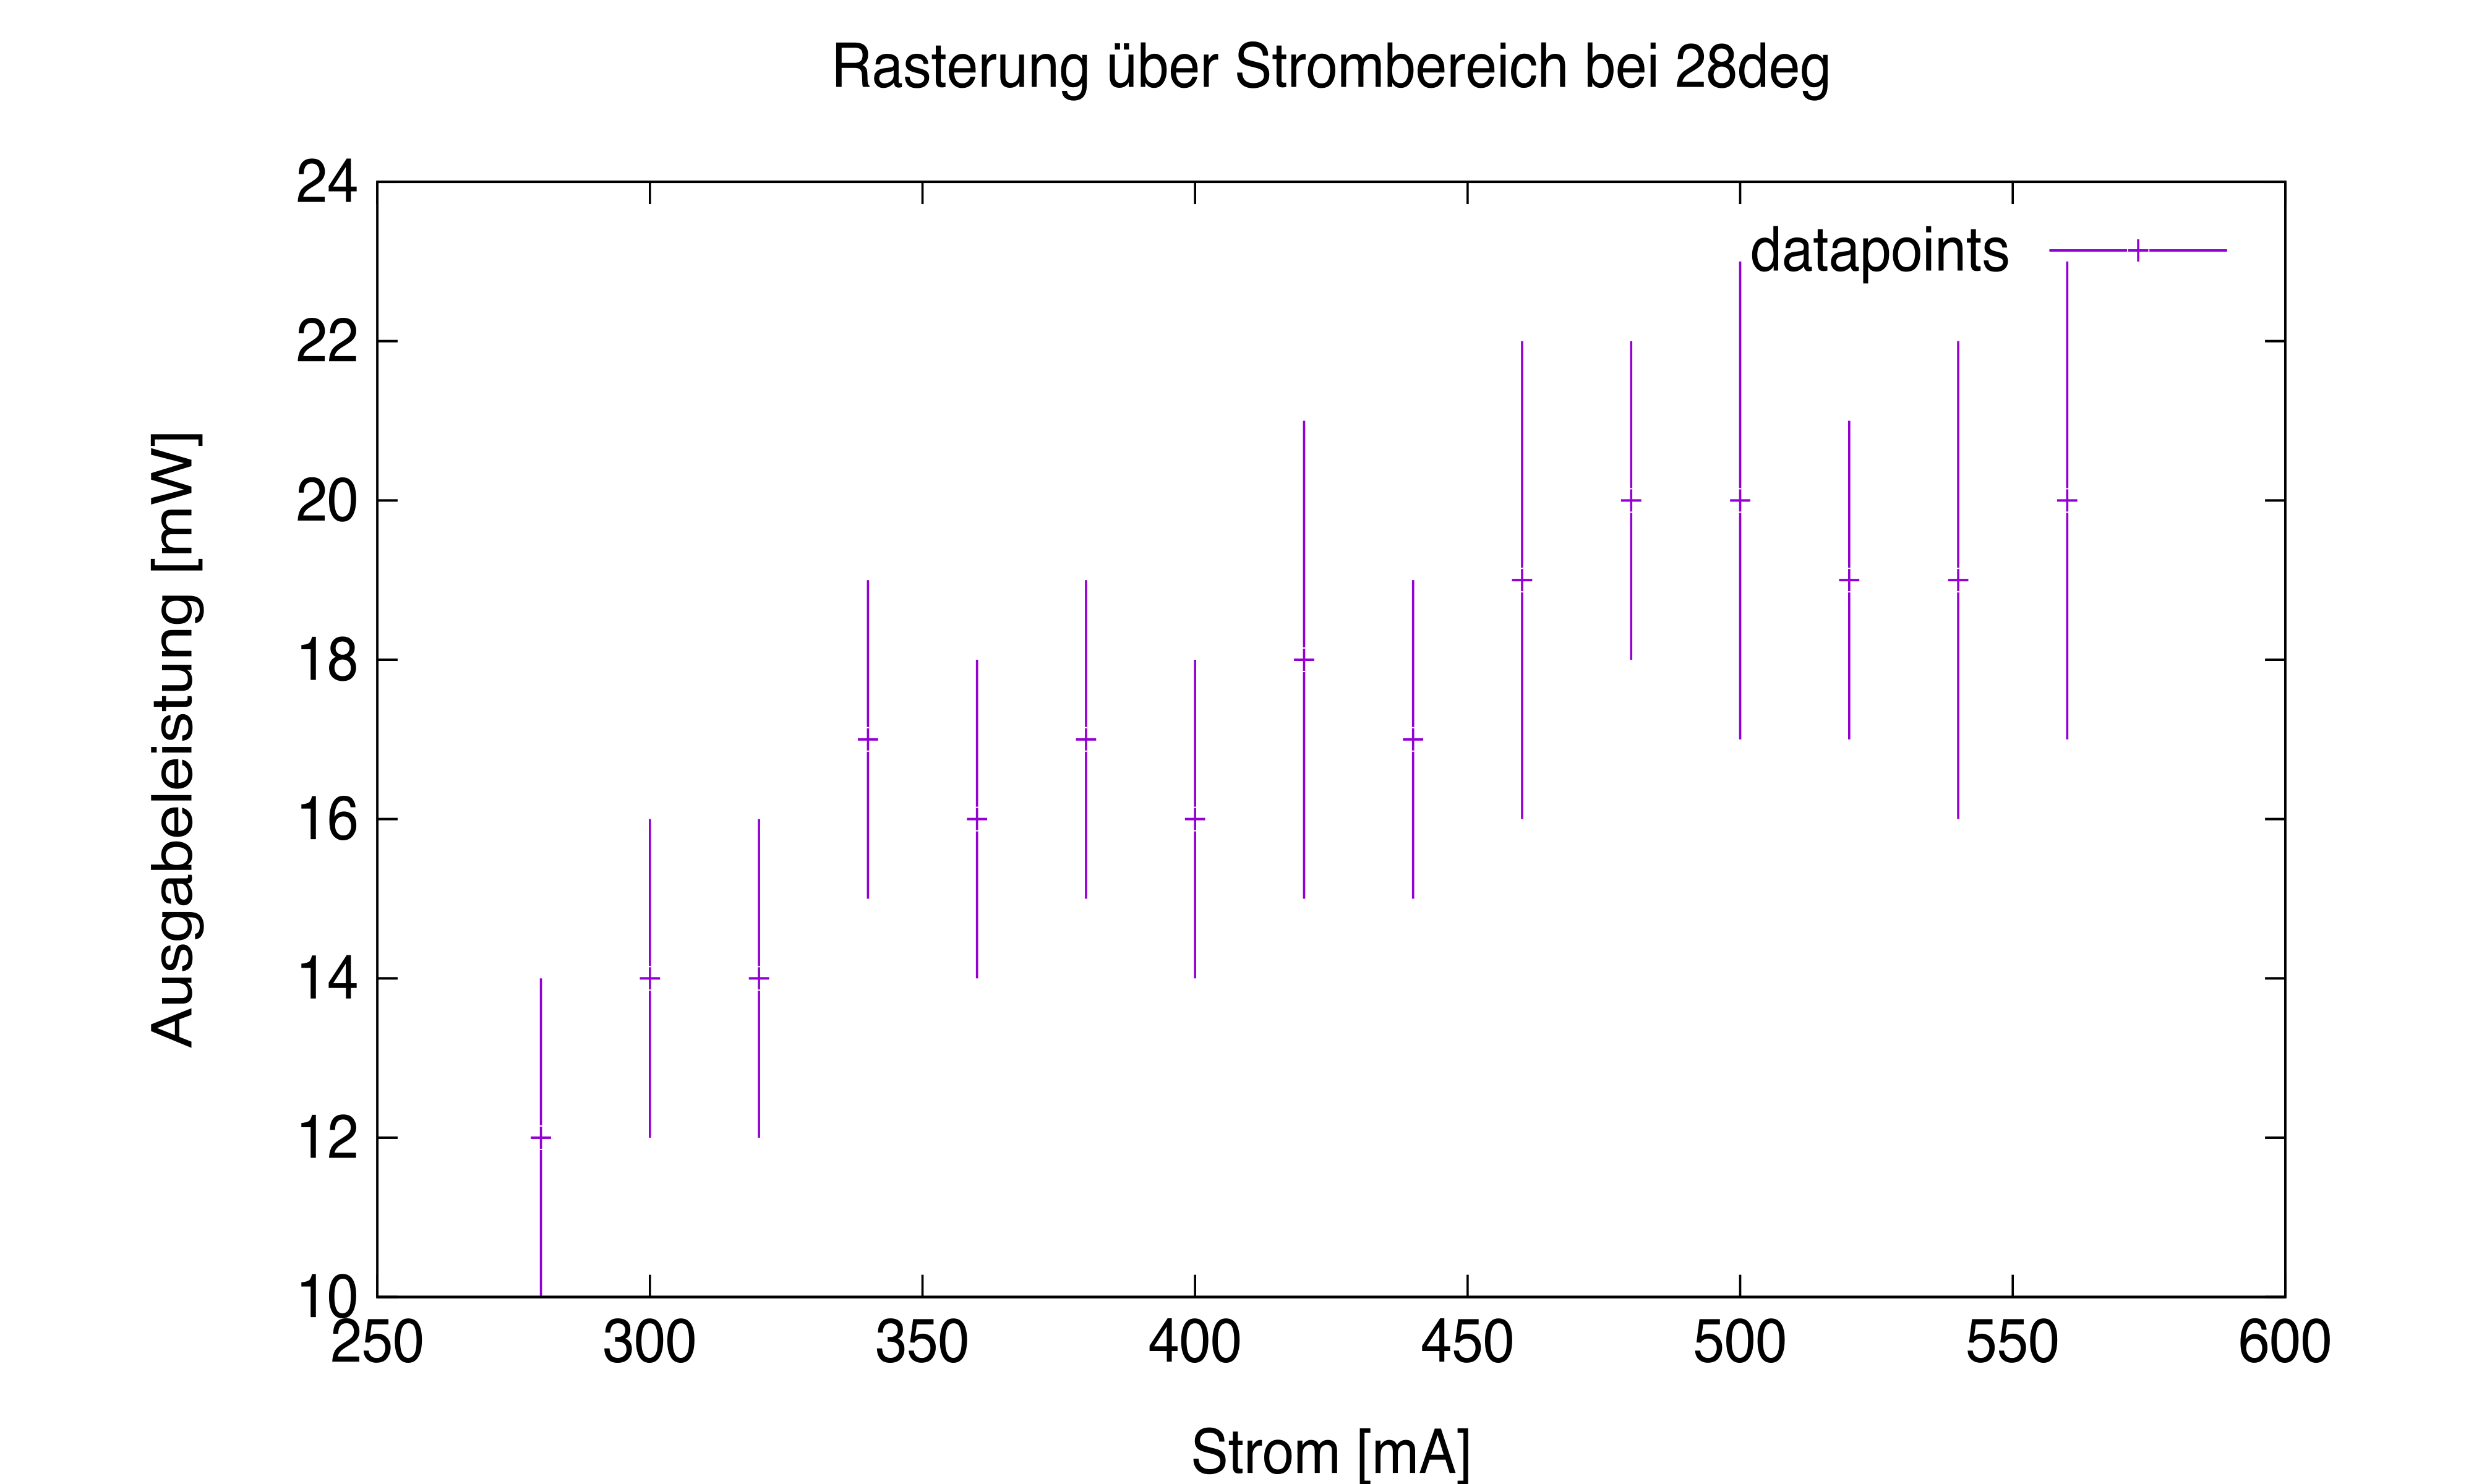
\includegraphics[width=\textwidth]{../../Bilddateien/1-2/Rasterung_28deg.png}
            \caption{Rasterung um $28\si{\celsius}$.}
            \label{fig:1-2:Rasterung28deg}
        \end{subfigure}
        \
        \begin{subfigure}[t]{0.45\textwidth}
            \centering
            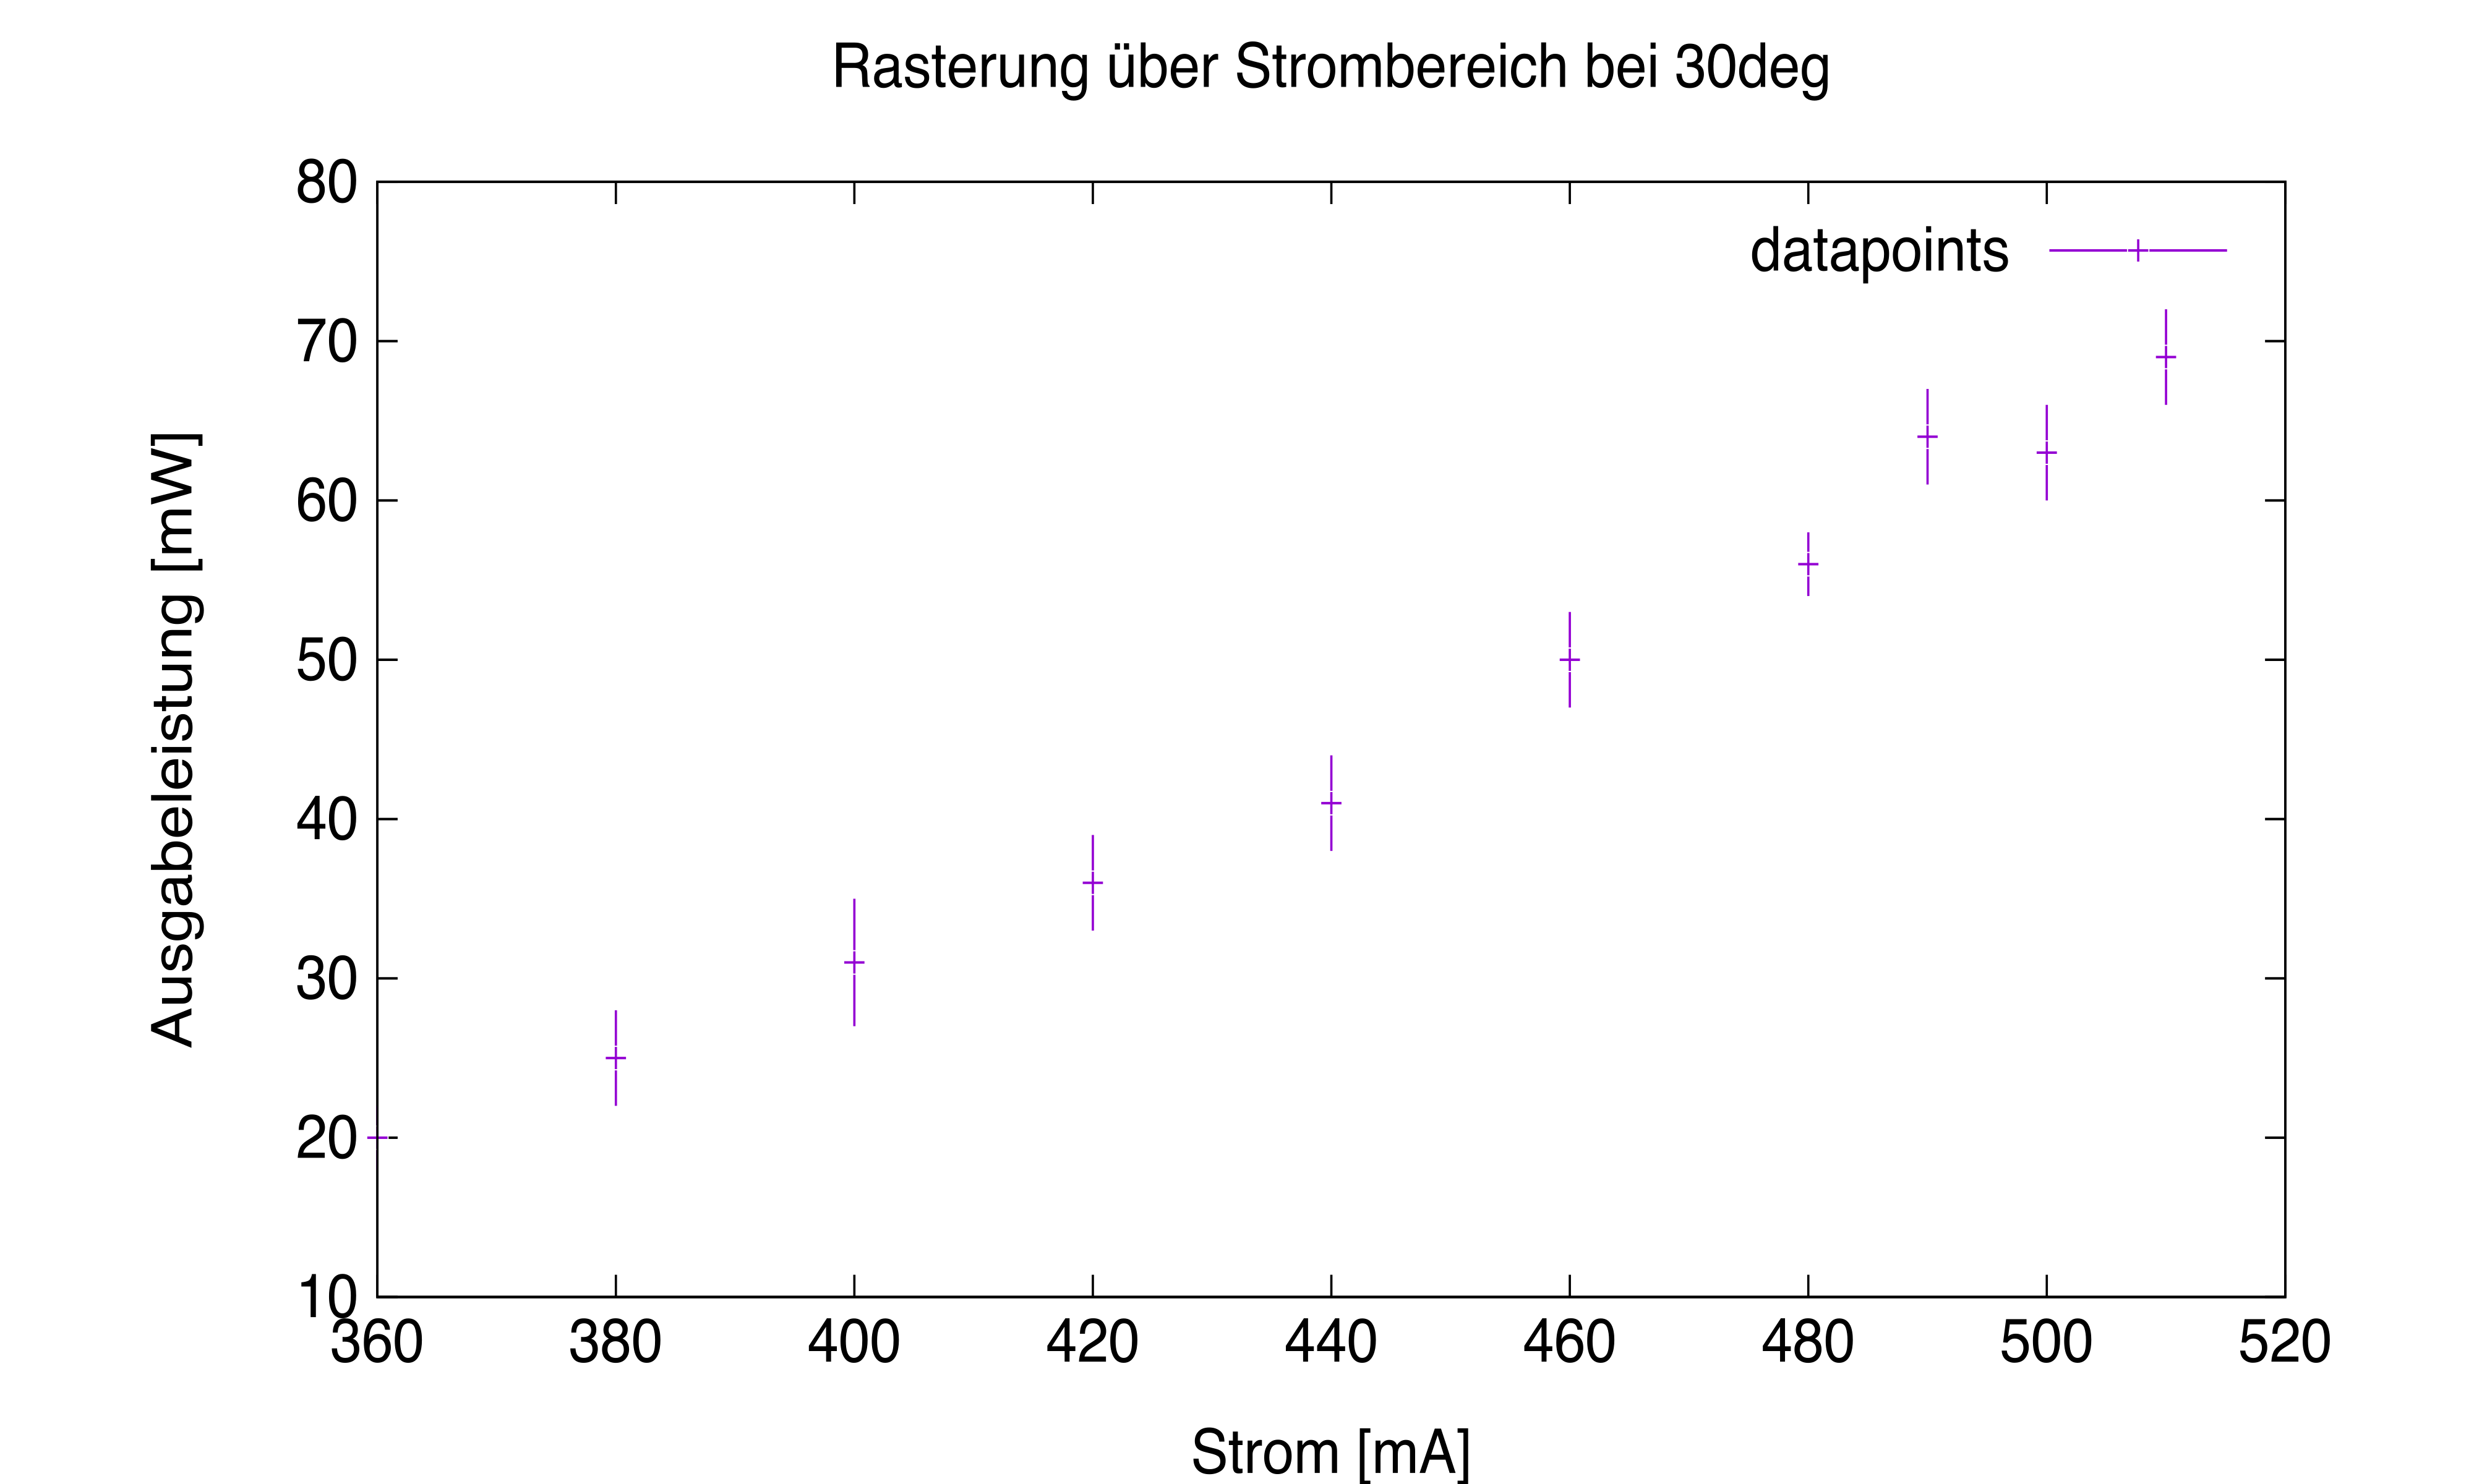
\includegraphics[width=\textwidth]{../../Bilddateien/1-2/Rasterung_30deg.png}
            \caption{Rasterung um $30\si{\celsius}$.}
            \label{fig:1-2:Rasterung30deg}
        \end{subfigure}
        \caption{Die Transmissionsleistung zu fester Temperatur $T\in\mcT$ als Funktion der Anregungsleistung $P_{\textit{an}}$.}
    \end{figure}

    Da wir jedoch durch große Schwankungen der Ausgabeleitung des ND:YAG Kristalls große Unsicherheiten vorfanden, wechselten wir das Verfahren zur Optimierung von $T\mapsto P_{\textit{an}}(T)$ mit Stromwerten $I_{\textit{an}}\in\{50\si{\mA},150\si{\mA},250\si{\mA},350\si{\mA},450\si{\mA},550\si{\mA}\}=:\mcI$, was durch die Proportionalität $I_{\textit{an}}\propto P_{\textit{an}}$ ebenfalls eine Charakterisierung der Kennlinie ermöglicht. Somit optimieren wir die Funktion
    \[
        I_{\textit{an}}\mapsto\textit{Tr}(P_{\textit{an}})(T_0(I_{\textit{an}}))
    \]
    und zeichnen zur Darstellung die Kennlinie als Funktion $I_{\textit{an}}\mapsto T_0(I_{\textit{an}})$ auf. Das Ergebnis der Messreihe ist in Abbildung \ref{fig:1-2:RasterungEvalMinChgI} gegeben. Eine Kurvenanpassung mittels linearen Zusammenhangs $f_{a,b}(x) := a\cdot x + b$ liefert uns die Parametertabelle \ref{tab:1-2:RasterungEvalMinChgI} mit Parametern $a,b$ und ihren zugehörig berechneten asymptotischen Standardunsicherheiten $u(a),u(b)$.

    \begin{figure}[H]
        \centering
        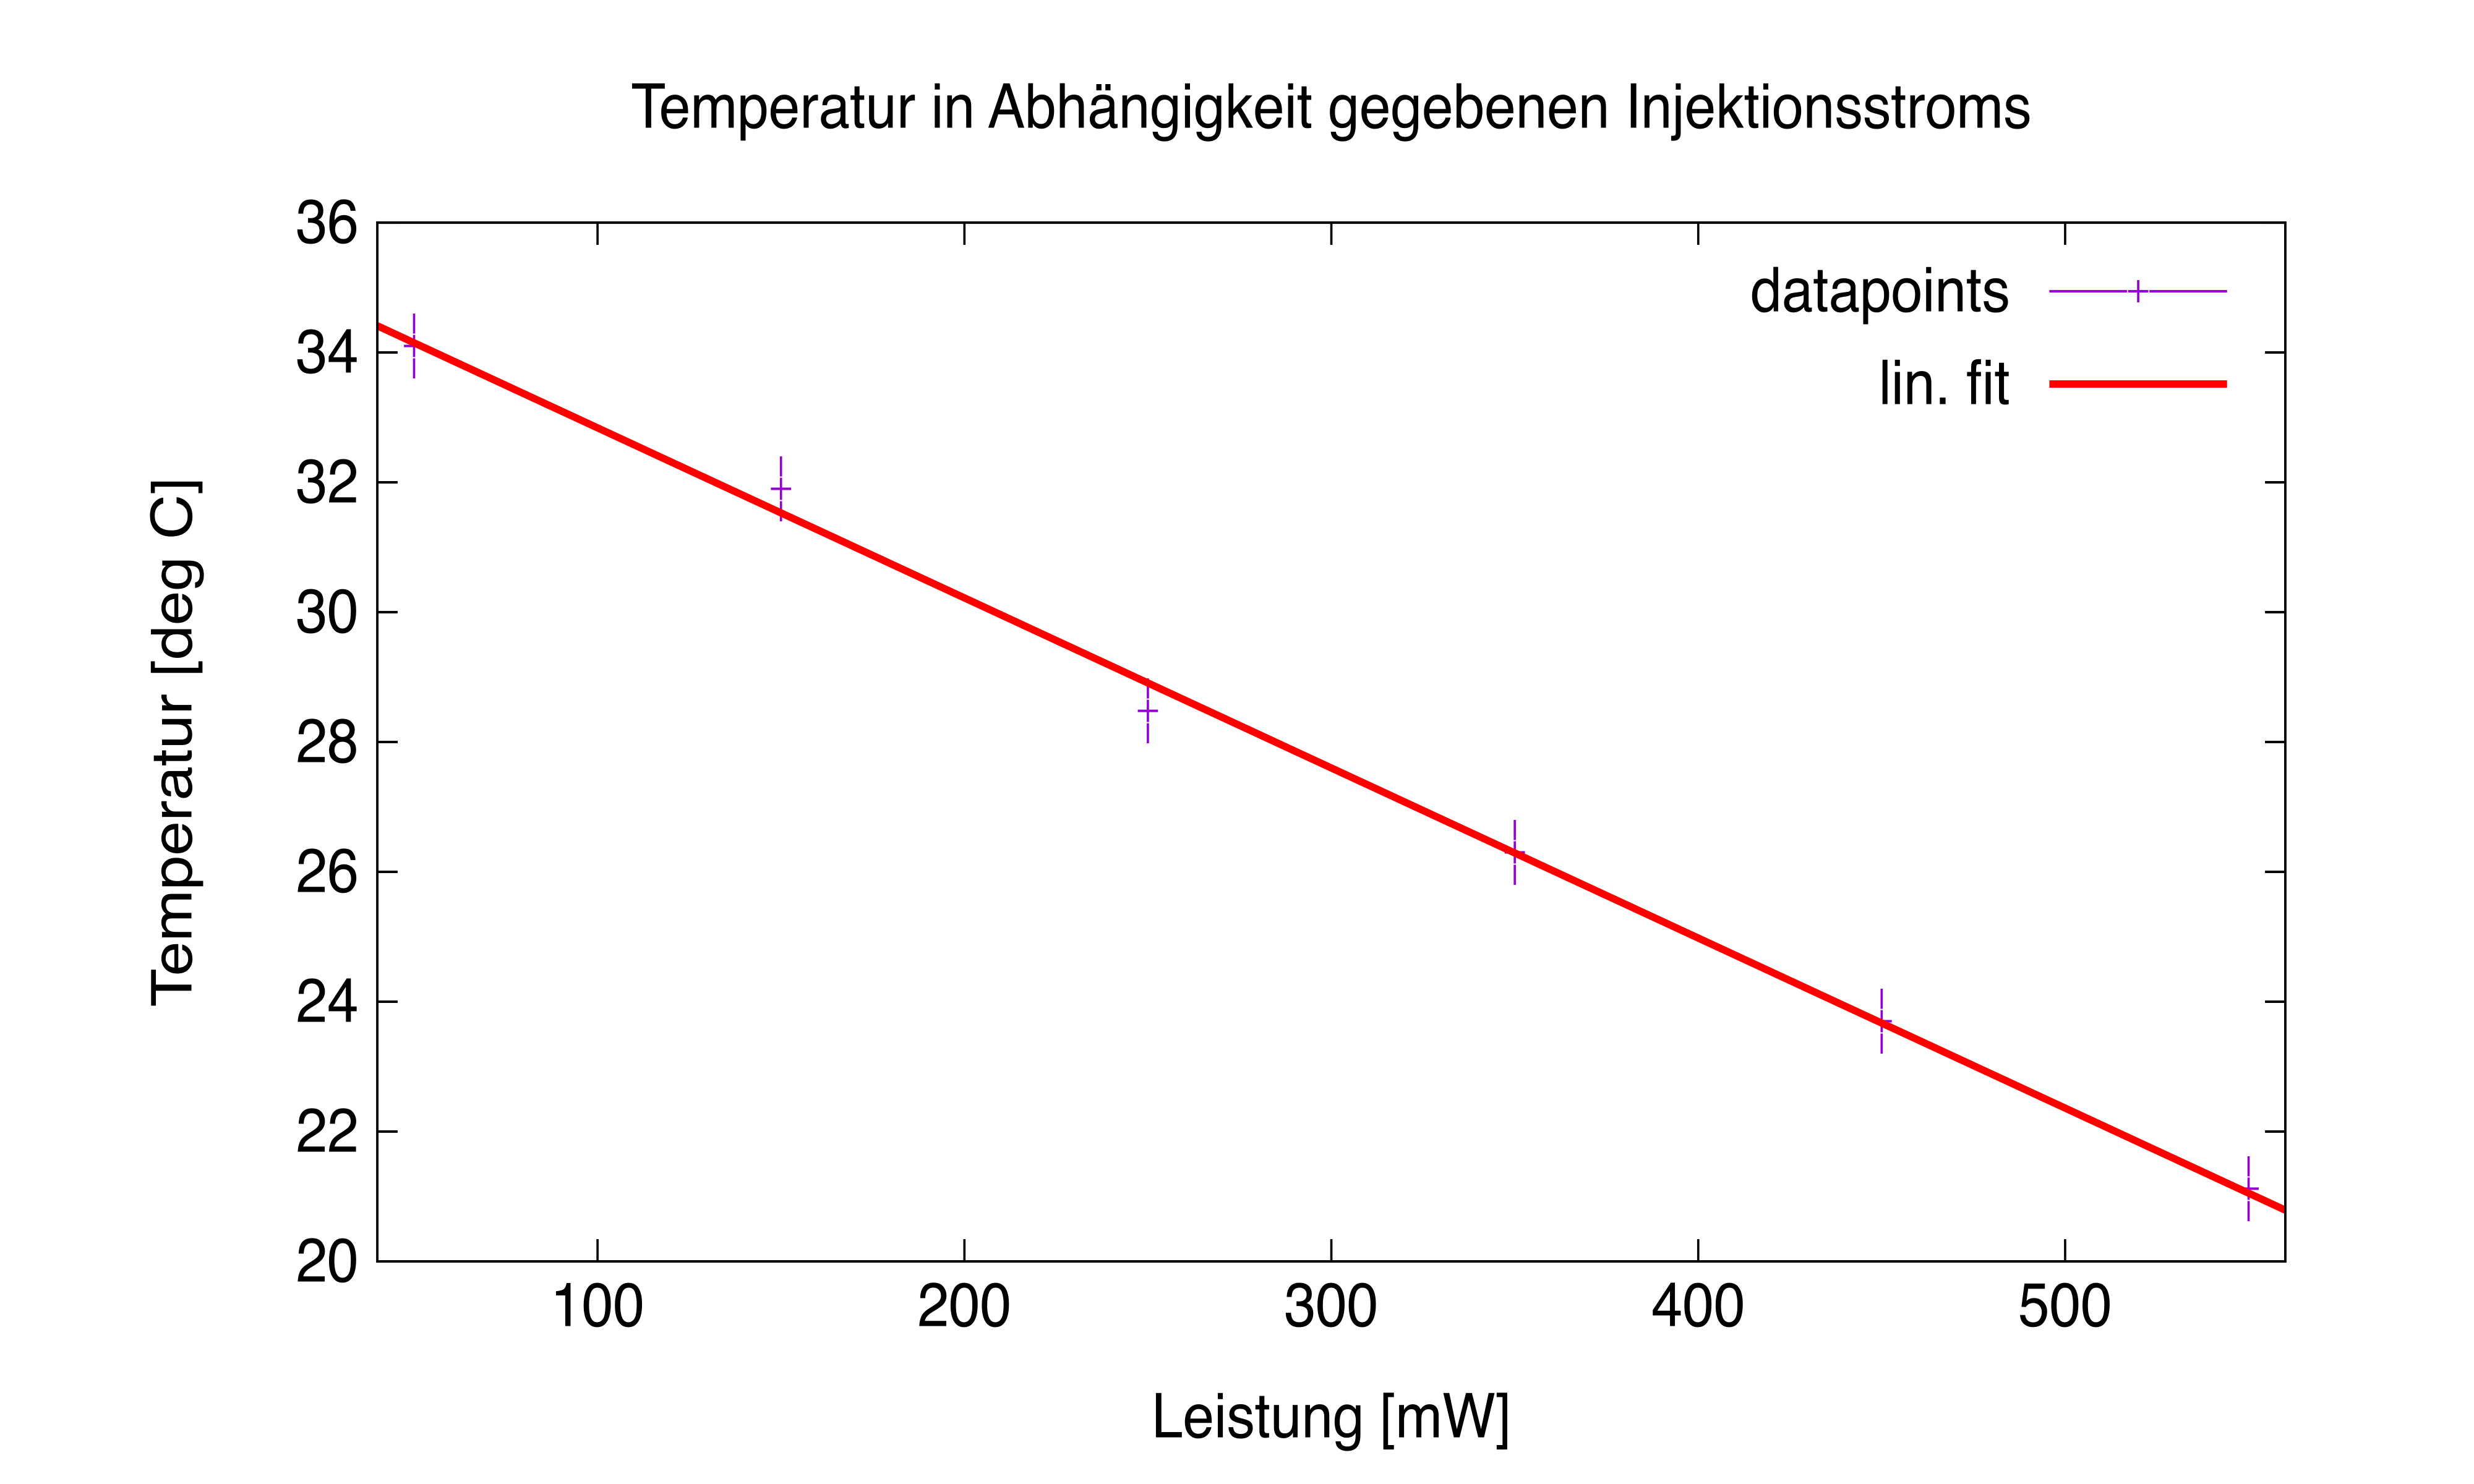
\includegraphics[width=11cm]{../../Bilddateien/1-2/Rasterung_EvalMin_chgI.png}
        \caption{Die optimierende Temperatur $T_0$ als Funktion des Anregungsstroms $I_{\textit{an}}$.}
        \label{fig:1-2:RasterungEvalMinChgI}
    \end{figure}

    \begin{table}[H]
        \centering
        \begin{tabular}{c|cc|cc}
            \hline
            & $a$ in $\si{\celsius\per\mW}$ & $u(a)$ in $\si{\celsius\per\mW}$ & $b$ in $\si{\celsius}$ & $u(b)$ in $\si{\celsius}$ \\
            \hline\hline
            $f_{a,b}$ & $-0.0261943$ & $0.0006868$ & $35.4583$ & $0.2371$ \\
            \hline
        \end{tabular}
    \end{table}
    Wir erkennen durch einen Quotientenvergleich $u(a)/a \approx 2.622\si{\percent}$ und $u(b)/b \approx 0.6686\si{\percent}$ eine gute Approximation der Messwerte. 
\end{document}